\section{Training and Development}
TVS : \\
\textbf{P1:} businesses should conduct and govern themselves with integrity, and in a manner that is ethical, transparent and accountable \\\textbf{P2:} businesses should provide goods and services in a manner that is sustainable and safe \\\textbf{P3:} businesses should respect and promote the well-being of all employees, including those in their value chains\\
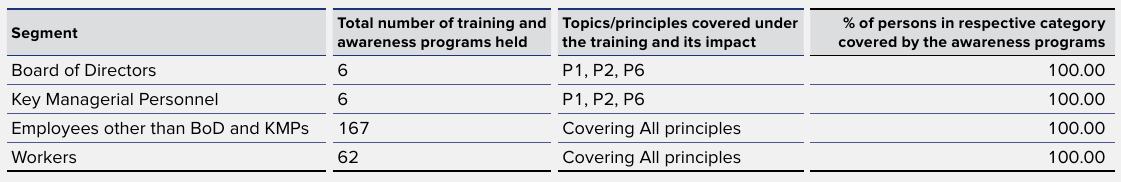
\includegraphics[width=\linewidth]{psycho_images/TVS_Training.png}\\
\textbf{Institute of Quality and Leadership (IQL)}: Offers programs in AR, VR, and digital simulations.\\
\textbf{Skill Enhancement}: Programs in R\&D, manufacturing excellence, and customer service.\\
\textbf{Leadership Development}: Mentoring, coaching, and strategic initiatives for leadership growth.\\\\
Hero: \\
11,18,505 Total training hours\\
32.93 Average training hours / employee\\
Rs 10,488 Average spent on training and development per employee (includes staff and permanent workers)\\
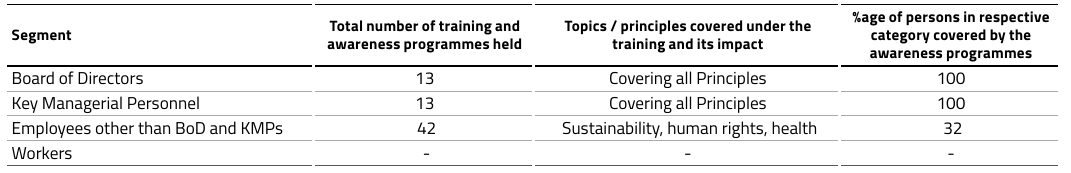
\includegraphics[width=\linewidth]{psycho_images/Hero_Training.png}\\\\
\textbf{Technical Training}: Programmes like CNC programming, auto-gauging, hydraulics, pneumatics, electrical, drives,	Integrated Management System (IMS) awareness, Total Productive Maintenance (TPM), Jishu Hozen (JH) pillar	awareness, and Kobetsu Kaizen (KK) pillar awareness for all segments of workforce.\\	
\textbf{Behavioural Training}: Training programmes which enhance
soft skills such as nurturing workplace relationships,
assertive communication, and Company’s core values
workshop. It also includes sensitisation programmes such
as POSH, gender sensitisation, unconscious bias, and
Code of Conduct.\\
\textbf{Functional Programmes}: Training programmes which
enable our workforce for upskilling data analytical
capacities like 7 QC tools training, Advanced Excel,
and Power BI.